\pdfminorversion=4
\documentclass[aspectratio=169]{beamer}

\mode<presentation>
{
  \usetheme{default}
  \usecolortheme{default}
  \usefonttheme{default}
  \setbeamertemplate{navigation symbols}{}
  \setbeamertemplate{caption}[numbered]
  \setbeamertemplate{footline}[frame number]  % or "page number"
  \setbeamercolor{frametitle}{fg=white}
  \setbeamercolor{footline}{fg=black}
} 

\usepackage[english]{babel}
\usepackage[utf8x]{inputenc}
\usepackage{tikz}
\usepackage{courier}
\usepackage{array}
\usepackage{bold-extra}
\usepackage{minted}
\usepackage[thicklines]{cancel}
\usepackage{fancyvrb}

\xdefinecolor{dianablue}{rgb}{0.18,0.24,0.31}
\xdefinecolor{darkblue}{rgb}{0.1,0.1,0.7}
\xdefinecolor{darkgreen}{rgb}{0,0.5,0}
\xdefinecolor{darkgrey}{rgb}{0.35,0.35,0.35}
\xdefinecolor{darkorange}{rgb}{0.8,0.5,0}
\xdefinecolor{darkred}{rgb}{0.7,0,0}
\definecolor{darkgreen}{rgb}{0,0.6,0}
\definecolor{mauve}{rgb}{0.58,0,0.82}

\title[2021-06-02-pyhepmod-jupyter-talk-talk]{Whatever}
\author{Jim Pivarski}
\institute{Princeton University -- IRIS-HEP}
\date{June 2, 2021}

\usetikzlibrary{shapes.callouts}

\begin{document}

\logo{\pgfputat{\pgfxy(0.11, 7.4)}{\pgfbox[right,base]{\tikz{\filldraw[fill=dianablue, draw=none] (0 cm, 0 cm) rectangle (50 cm, 1 cm);}\mbox{\hspace{-8 cm}
\includegraphics[height=1 cm]{princeton-logo-long.png}\hspace{0.1 cm}\raisebox{0.1 cm}{
\includegraphics[height=0.8 cm]{iris-hep-logo-long.png}}\hspace{0.1 cm}}}}}

\begin{frame}
  \titlepage
\end{frame}

\logo{\pgfputat{\pgfxy(0.11, 7.4)}{\pgfbox[right,base]{\tikz{\filldraw[fill=dianablue, draw=none] (0 cm, 0 cm) rectangle (50 cm, 1 cm);}\mbox{\hspace{-8 cm}
\includegraphics[height=1 cm]{princeton-logo.png}\hspace{0.1 cm}\raisebox{0.1 cm}{
\includegraphics[height=0.8 cm]{iris-hep-logo.png}}\hspace{0.1 cm}}}}}

% Uncomment these lines for an automatically generated outline.
%\begin{frame}{Outline}
%  \tableofcontents
%\end{frame}

% START START START START START START START START START START START START START

\begin{frame}{``Interactive computational notebook'' is not a new idea}
\vspace{0.25 cm}
\begin{columns}
\column{0.95\linewidth}
\centering\only<1>{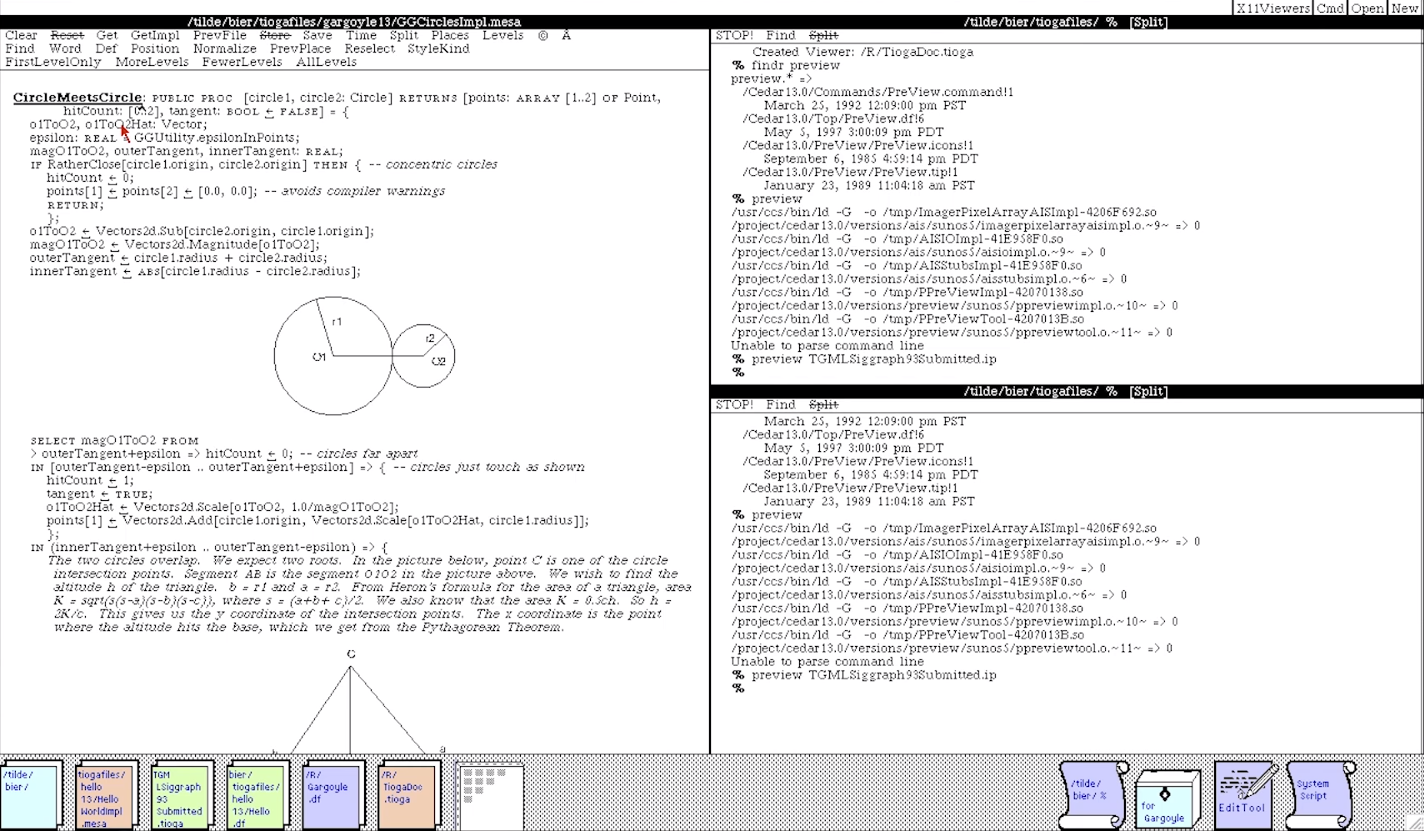
\includegraphics[height=7.5 cm]{img/screenshot-1982-cedar-tioga.png}}\only<2>{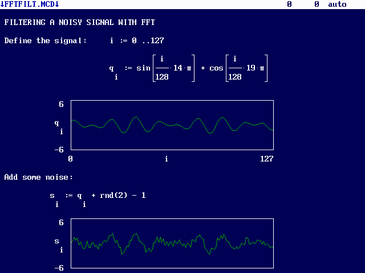
\includegraphics[height=7.5 cm]{img/screenshot-1986-mathcad.png}}\only<3>{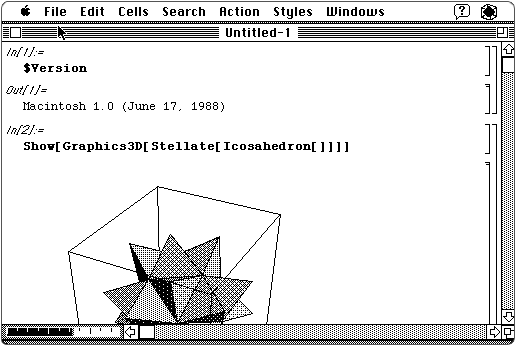
\includegraphics[height=7.5 cm]{img/screenshot-1987-mathematica.png}}\only<4>{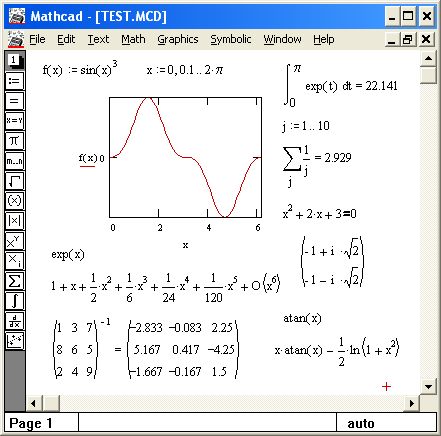
\includegraphics[height=7.5 cm]{img/screenshot-1992-mathcad.png}}\only<5>{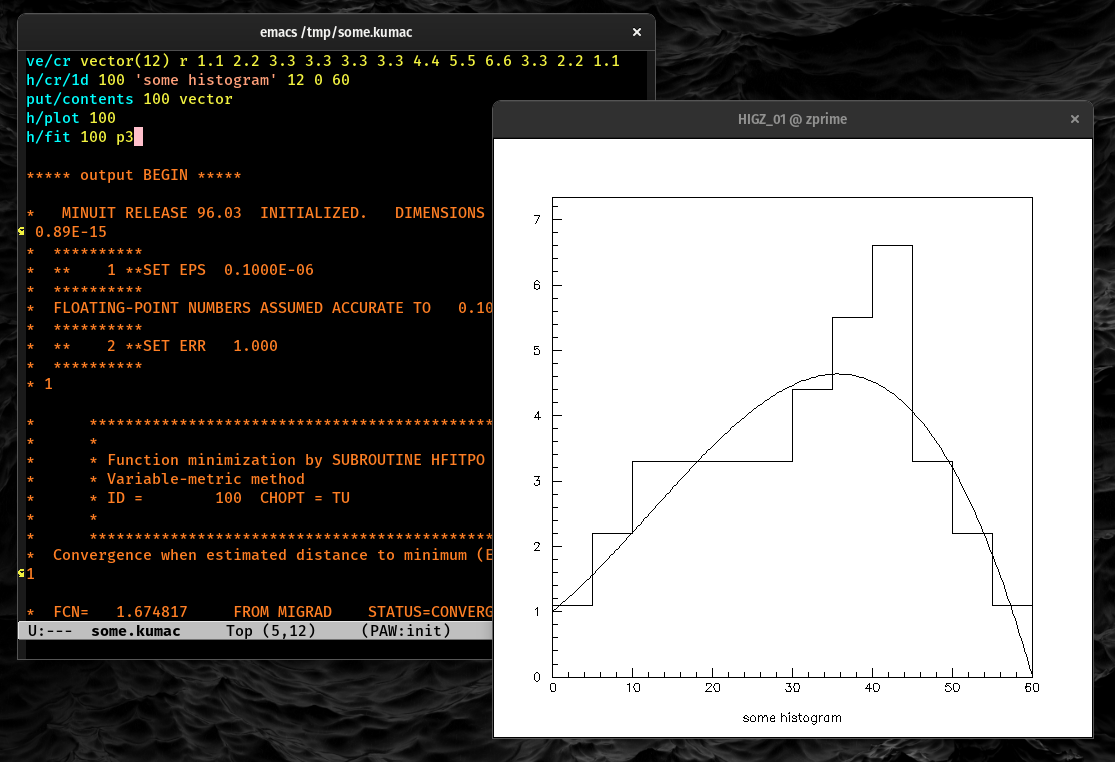
\includegraphics[height=7.5 cm]{img/screenshot-2000-paw-mode.png}}\only<6>{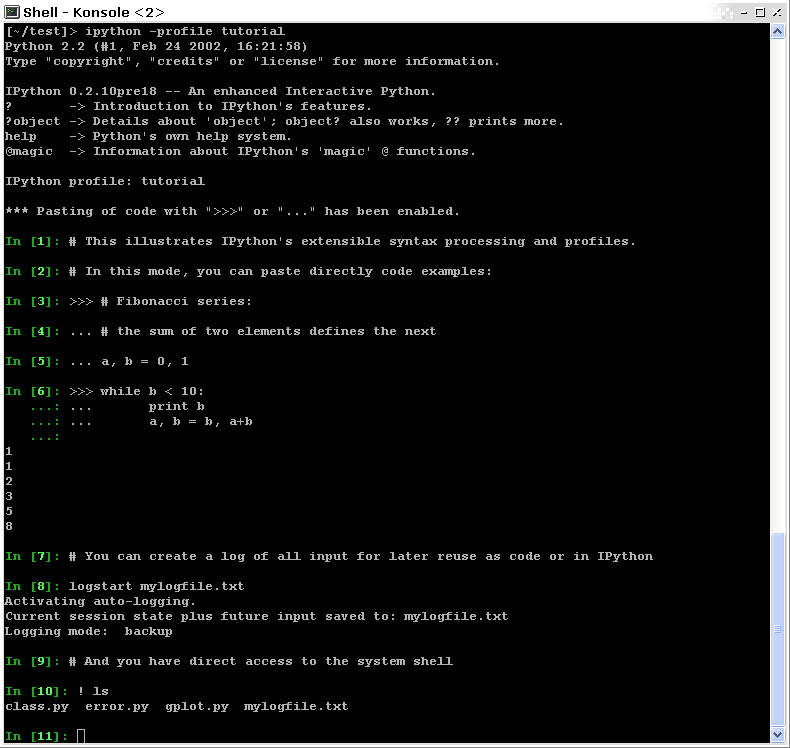
\includegraphics[height=7.5 cm]{img/screenshot-2002-ipython.png}}\only<7>{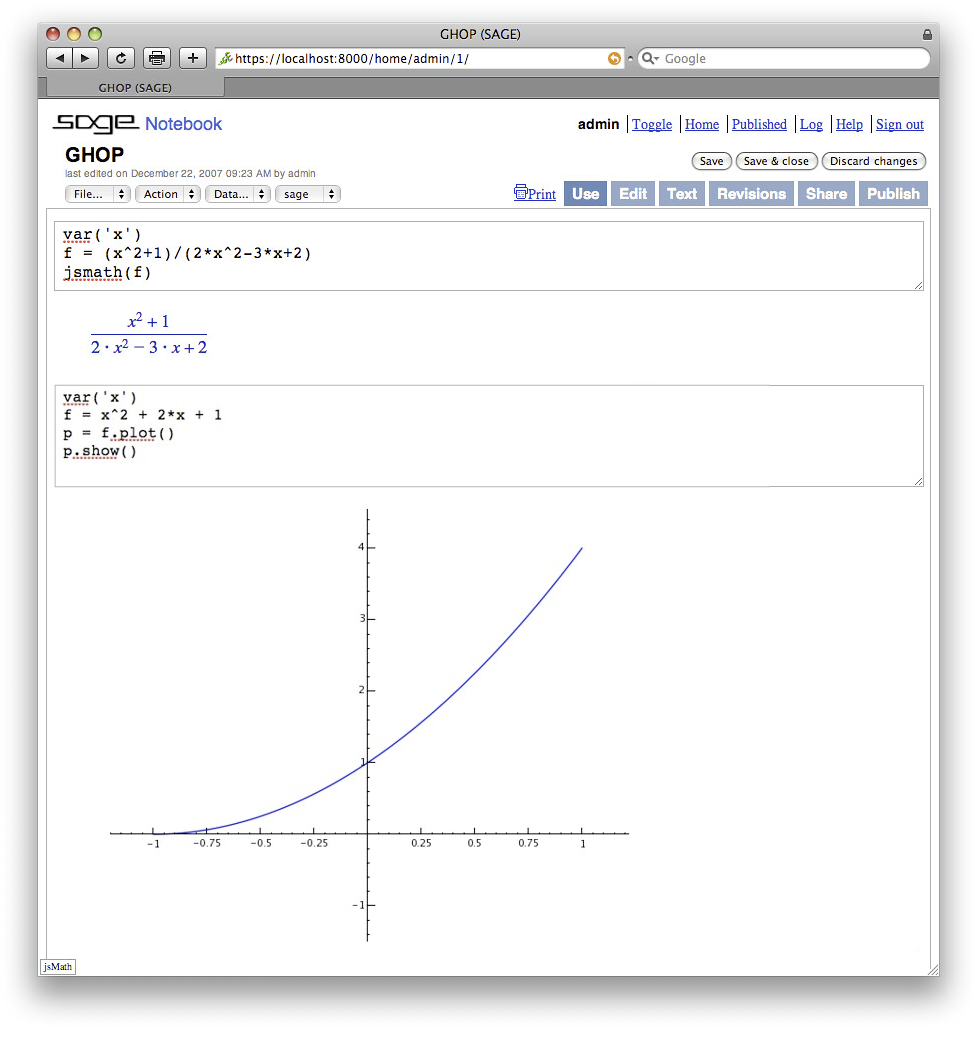
\includegraphics[height=7.5 cm]{img/screenshot-2007-sage.png}}\only<8>{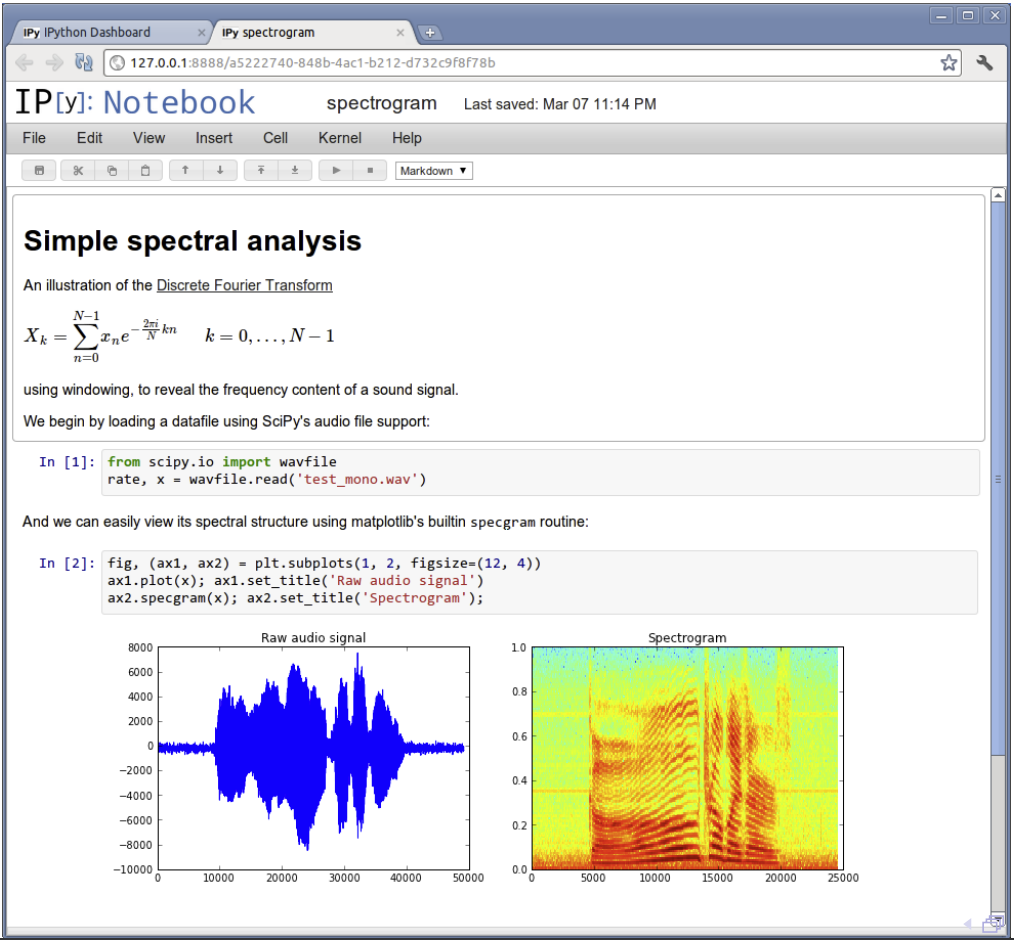
\includegraphics[height=7.5 cm]{img/screenshot-2012-ipython-notebook.png}}\only<9>{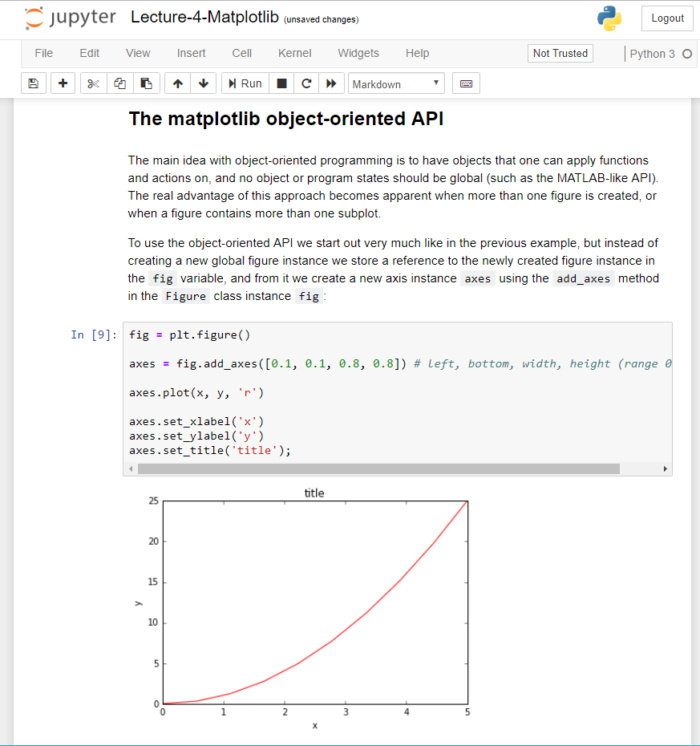
\includegraphics[height=7.5 cm]{img/screenshot-2015-jupyter-notebook.png}}\only<10>{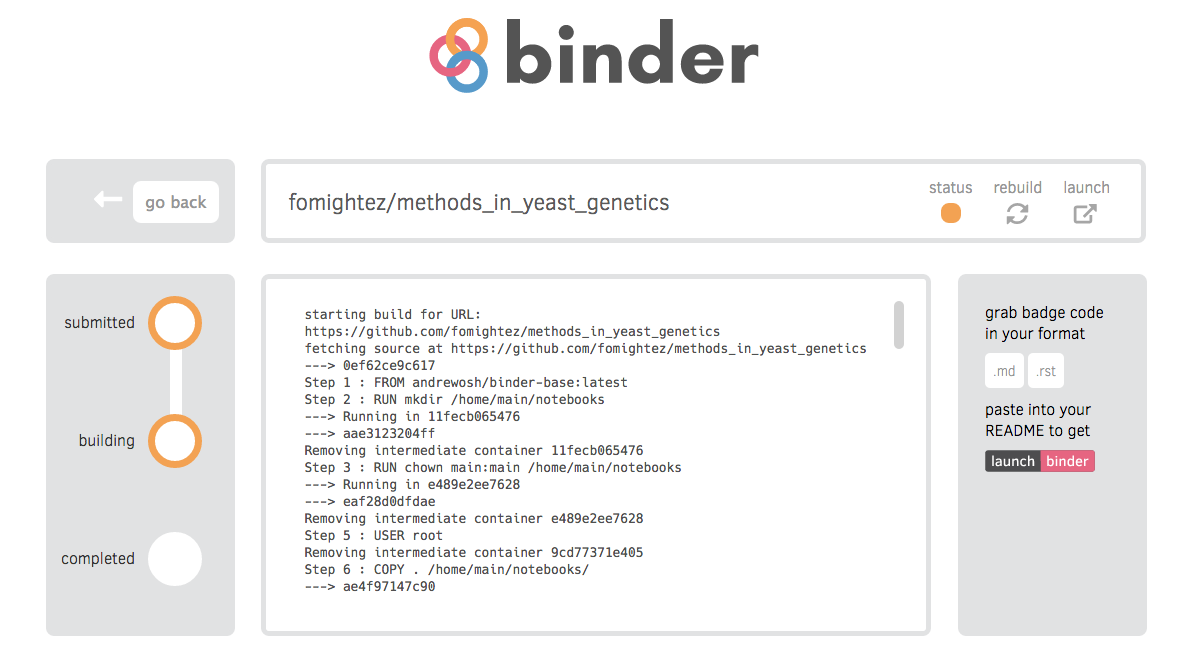
\includegraphics[height=7.5 cm]{img/screenshot-2016-binder.png}}\only<11>{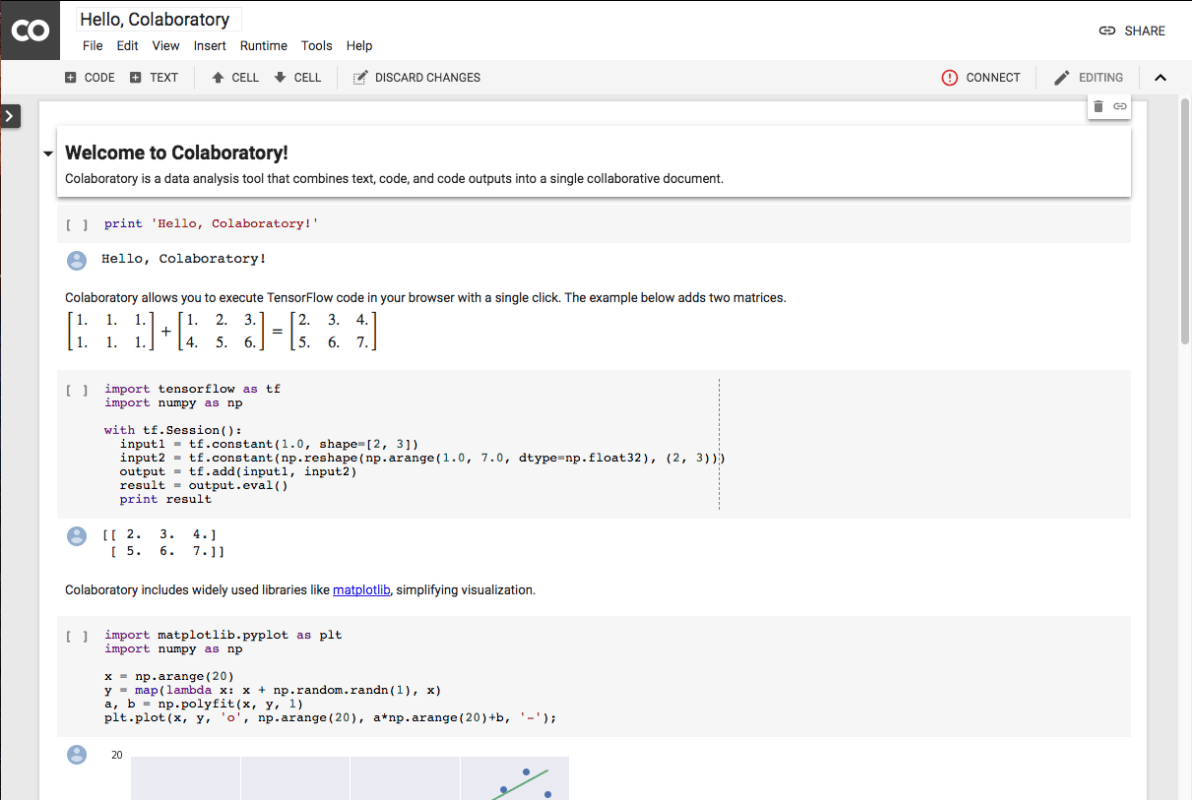
\includegraphics[height=7.5 cm]{img/screenshot-2018-colab.png}}\only<12>{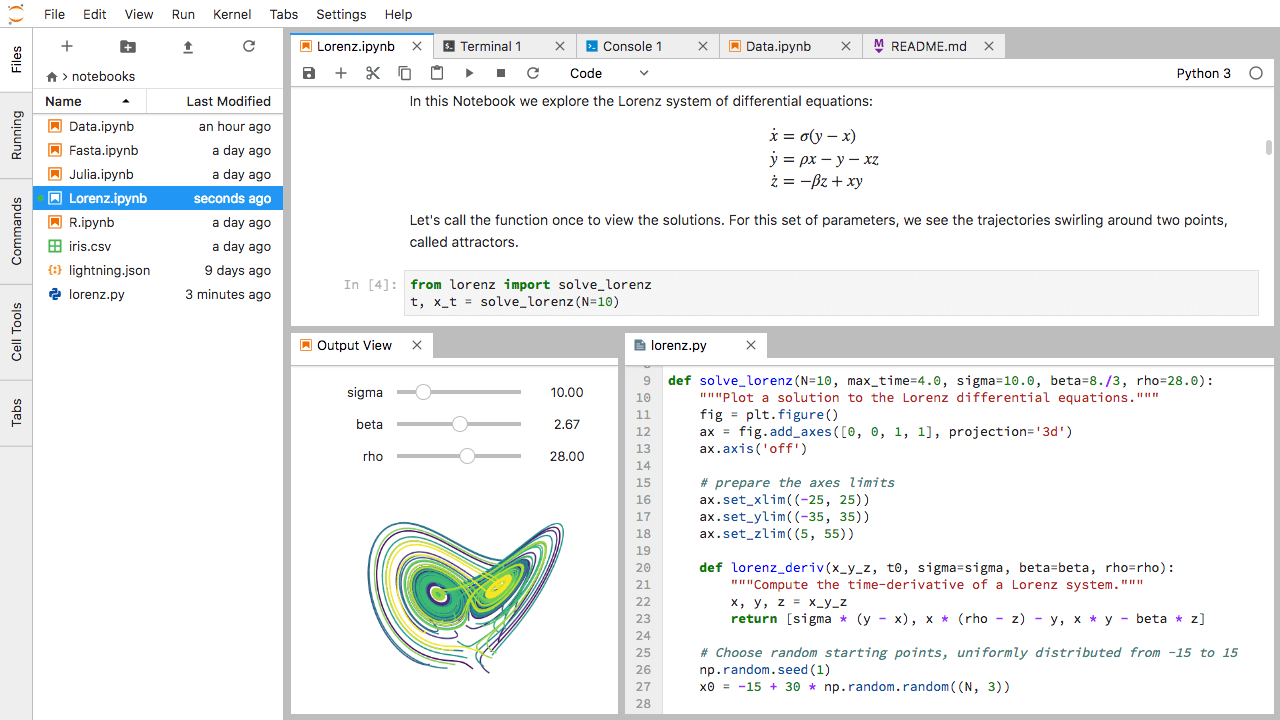
\includegraphics[height=7.5 cm]{img/screenshot-2018-jupyterlab.png}}\only<13>{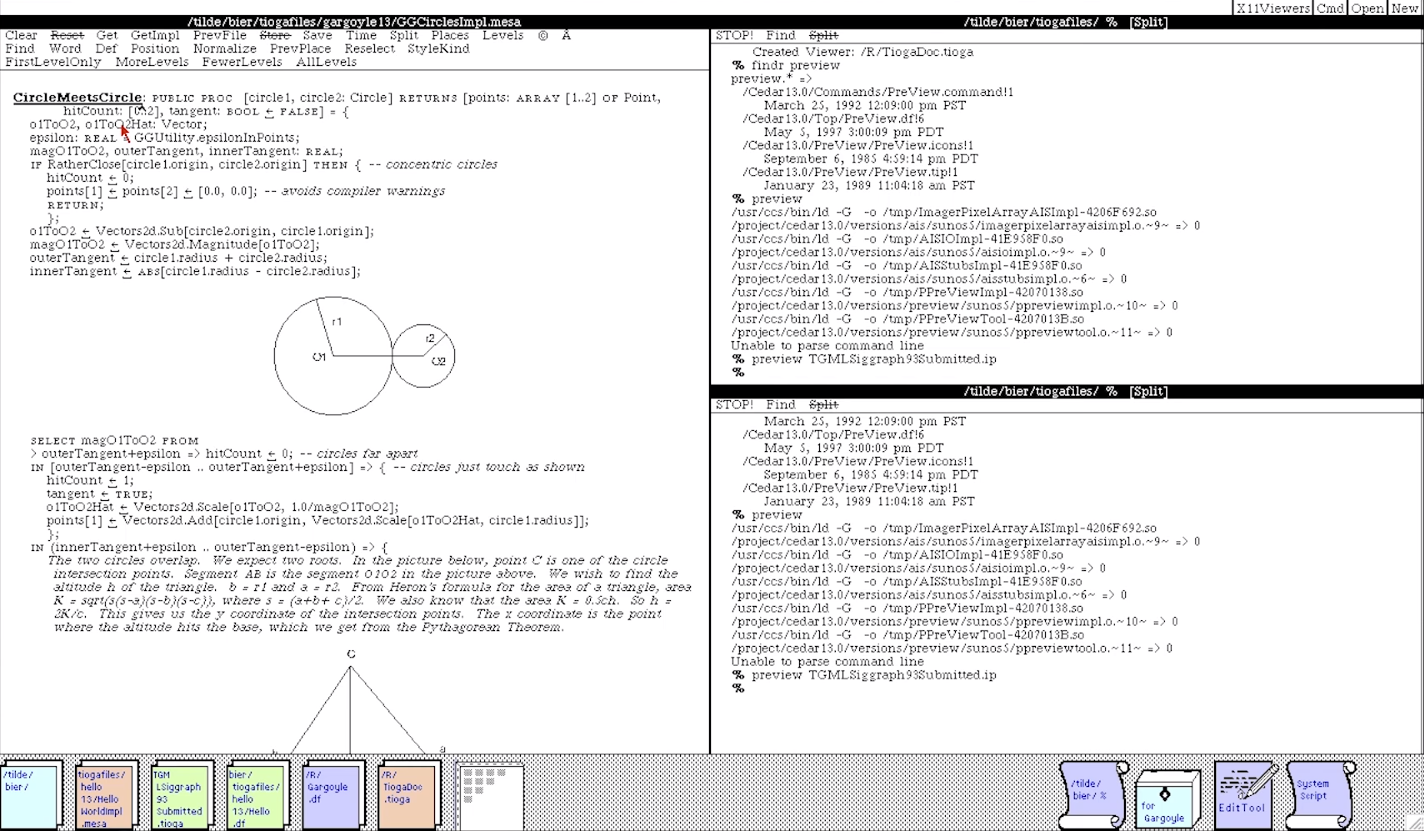
\includegraphics[height=7.5 cm]{img/screenshot-1982-cedar-tioga.png}}

\column{0.15\linewidth}
\LARGE
\only<1>{1982}\only<2>{1986}\only<3>{1987}\only<4>{1992}\only<5>{2000}\only<6>{2002}\only<7>{2007}\only<8>{2012}\only<9>{2015}\only<10>{2016}\only<11>{2018}\only<12>{2018}\only<13>{\mbox{ }}

\normalsize
\vspace{0.25 cm}
\only<1>{Xerox's \textcolor{darkblue}{Tioga} editor for the Cedar language

\vspace{0.25 cm}
(Xerox-PARC invented everything GUI-related)}\only<2>{\textcolor{darkblue}{Mathcad}, first computational notebook to run on PCs}\only<3>{\textcolor{darkblue}{Mathematica}}\only<4>{\textcolor{darkblue}{Mathcad} again (on Windows)}\only<5>{\textcolor{darkblue}{PAW-mode} for Emacs (number of users = 1)}\only<6>{\textcolor{darkblue}{iPython}: cell-based Python in the terminal}\only<7>{\textcolor{darkblue}{SAGE}: cell-based Python in a web browser}\only<8>{\textcolor{darkblue}{iPython-notebook}: cell-based Python in a web browser

\vspace{0.25 cm}
But popular this time!}\only<9>{\textcolor{darkblue}{Jupyter}: rebranding to emphasize multi-language support

\vspace{0.25 cm}
{\bf Ju}lia $+$

{\bf Py}thon $+$

{\bf R}}\only<10>{\textcolor{darkblue}{Binder}: Jupyter notebooks on the cloud}\only<11>{\textcolor{darkblue}{Google Colab}: Jupyterish notebooks on the cloud}\only<12>{\textcolor{darkblue}{JupyterLab}: fully featured editor environment

\vspace{0.25 cm}
Now it's starting to look like Tioga\ldots}\only<13>{a bit\ldots}
\end{columns}
\end{frame}

\begin{frame}{Jupyter is now mainstream}
\vspace{0.5 cm}
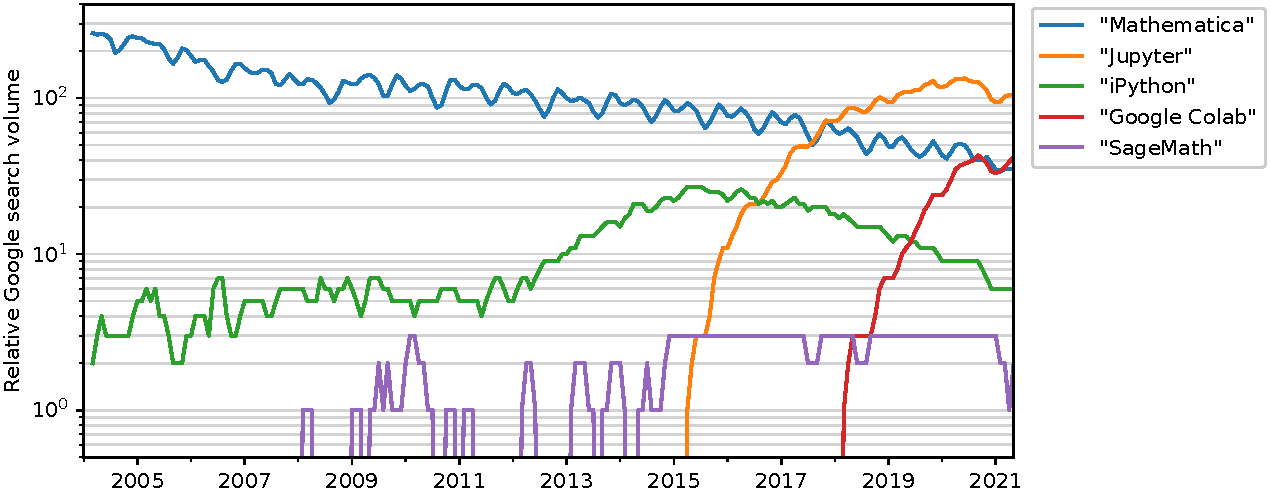
\includegraphics[width=\linewidth]{img/trends-jupyter-ipython.pdf}
\end{frame}


\end{document}
